\section{Impactos no mercado de psicologia}
\label{sec:impactoPsicologia}

A pesquisa realizada pela \citeonline{ABP2020}, levou em conta médicos psiquiatras ligados à associação e constatou que cerca de 47\% dos entrevistados relataram aumento em seus atendimentos após o início da pandemia, deste grupo, para cerca de um terço dos entrevistados, os atendimentos cresceram em até 25\%.

Diante da perspectiva de aumento, a pesquisa também citou que cerca de 68\% dos entrevistados receberam pacientes novos, que nunca haviam apresentado sintomas psiquiátricos antes. Além disso, 69\% dos profissionais também relataram que voltaram a atender pacientes que já haviam recebido alta médica e que retornaram ao consultório com reincidência de seus sintomas.

Já para o grupo de profissionais que não perceberam aumento em seus atendimentos, cerca de 45\% dos entrevistados discursaram justamente ao movimento contrário, a de queda em seus atendimentos. Dentre os motivos listados, o de maior destaque está na interrupção do tratamento por parte do paciente, devido às problemáticas de contato da pandemia.

Em outro âmbito, a pesquisa \textit{COVID-19 Practitioner Impact Survey}, realizada pela \citeonline{Association2022}, que levou em consideração profissionais licenciados dos Estados Unidos, relatou que cerca de 38\% dos profissionais constataram estar trabalhando mais em relação ao início da pandemia. Nesse mesmo contexto, cerca de 43\% dos entrevistados relataram estarem atendendo mais pacientes em comparação ao período anterior da pandemia, onde em média, 15.7 pessoas contatam o profissional por mês(excluindo os que já são pacientes).

Por fim, segundo a pesquisa, tamanho crescimento do mercado extrapola-se em outra tendência do mercado, cerca de 4 em cada 10 psicólogos (38\%) relatam manter uma lista de espera com tamanhos variados, onde 58\% são listas de até 9 pessoas e 20\% são listas de 10 até 19 pessoas.

\begin{figure}[H]
    \centering
    \caption{Número de pessoas me fila de espera para atendimento psicológico}
    \label{fig:listaDeEspera}
    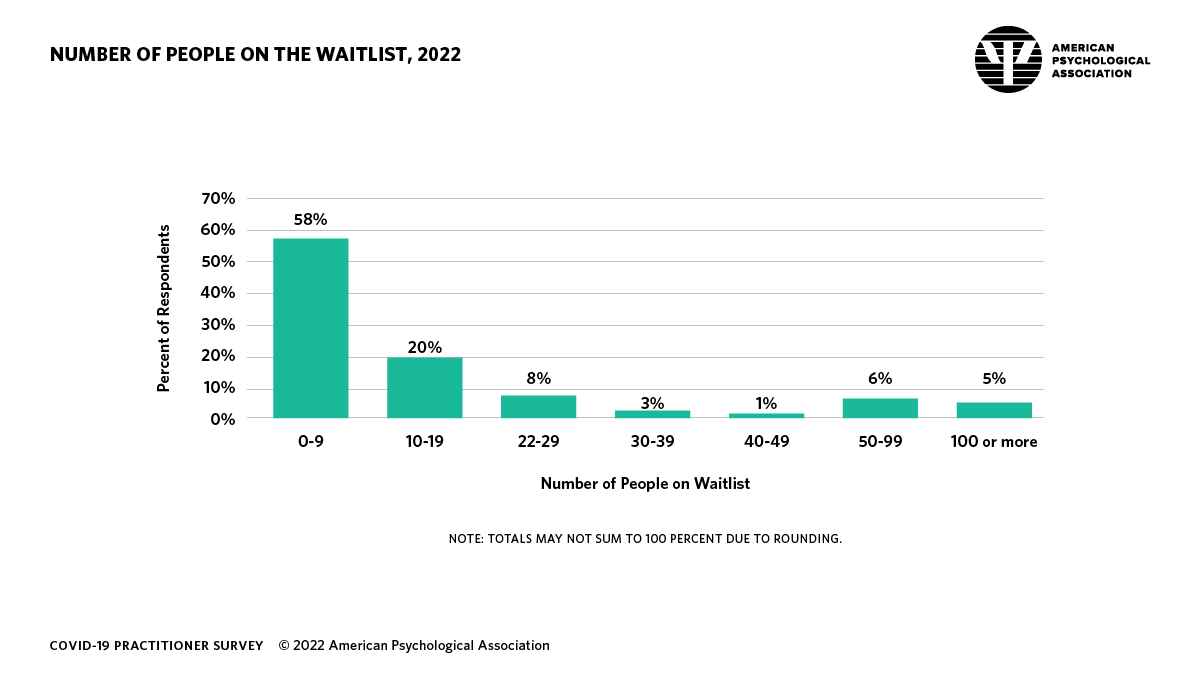
\includegraphics[width=.9\textwidth]{data/figures/lista-de-espera-psicologia.png}
    \fonte{\cite{Association2022}}
\end{figure}